\documentclass{beamer}
\mode<presentation>
\usepackage{amsmath}
\usepackage{amssymb}
%\usepackage{advdate}
\usepackage{adjustbox}
\usepackage{subcaption}
\usepackage{enumitem}
\usepackage{multicol}
\usepackage{mathtools}
\usepackage{listings}
\usepackage{url}
\def\UrlBreaks{\do\/\do-}
\usetheme{Frankfurt}
%\usecolortheme{lily}
\setbeamertemplate{footline}
{
	\leavevmode%
	\hbox{%
		\begin{beamercolorbox}[wd=\paperwidth,ht=2.25ex,dp=1ex,right]{author in head/foot}%
			\insertframenumber{} / \inserttotalframenumber\hspace*{2ex} 
		\end{beamercolorbox}}%
		\vskip0pt%
	}
	\setbeamertemplate{navigation symbols}{}

	\providecommand{\nCr}[2]{\,^{#1}C_{#2}} % nCr
	\providecommand{\nPr}[2]{\,^{#1}P_{#2}} % nPr
	\providecommand{\mbf}{\mathbf}
	\providecommand{\pr}[1]{\ensuremath{\Pr\left(#1\right)}}
	\providecommand{\qfunc}[1]{\ensuremath{Q\left(#1\right)}}
	\providecommand{\sbrak}[1]{\ensuremath{{}\left[#1\right]}}
	\providecommand{\lsbrak}[1]{\ensuremath{{}\left[#1\right.}}
	\providecommand{\rsbrak}[1]{\ensuremath{{}\left.#1\right]}}
	\providecommand{\brak}[1]{\ensuremath{\left(#1\right)}}
	\providecommand{\lbrak}[1]{\ensuremath{\left(#1\right.}}
	\providecommand{\rbrak}[1]{\ensuremath{\left.#1\right)}}
	\providecommand{\cbrak}[1]{\ensuremath{\left\{#1\right\}}}
	\providecommand{\lcbrak}[1]{\ensuremath{\left\{#1\right.}}
	\providecommand{\rcbrak}[1]{\ensuremath{\left.#1\right\}}}
	\theoremstyle{remark}
	\newtheorem{rem}{Remark}
	\newcommand{\sgn}{\mathop{\mathrm{sgn}}}
	\providecommand{\abs}[1]{\left\vert#1\right\vert}
	\providecommand{\res}[1]{\Res\displaylimits_{#1}} 
	\providecommand{\norm}[1]{\lVert#1\rVert}
	\providecommand{\mtx}[1]{\mathbf{#1}}
	\providecommand{\mean}[1]{E\left[ #1 \right]}
	\providecommand{\fourier}{\overset{\mathcal{F}}{ \rightleftharpoons}}
	%\providecommand{\hilbert}{\overset{\mathcal{H}}{ \rightleftharpoons}}
	\providecommand{\system}{\overset{\mathcal{H}}{ \longleftrightarrow}}
	%\newcommand{\solution}[2]{\textbf{Solution:}{#1}}
	%\newcommand{\solution}{\noindent \textbf{Solution: }}
	\providecommand{\dec}[2]{\ensuremath{\overset{#1}{\underset{#2}{\gtrless}}}}
	\newcommand{\myvec}[1]{\ensuremath{\begin{pmatrix}#1\end{pmatrix}}}
		\let\vec\mathbf

		\lstset{
			%language=C,
			frame=single, 
			breaklines=true,
			columns=fullflexible
		}

		\numberwithin{equation}{section}

\title{Gradient Descent}
\author{Faraz Patnam,\\ EE24BTECH11049,\\IIT Hyderabad.\\}

\date{\today} 
\begin{document}

\begin{frame}{Title}
    \titlepage
\end{frame}

\section*{Table of Contents}
\begin{frame}
    \tableofcontents
\end{frame}

\section{Problem Statement}
\begin{frame}{Question}
    \textbf{Question:}\\
A wire of length 28 m is to be cut into two pieces. One of the pieces is to be made into a square and the other into a circle. What should be the length of the two pieces so that the combined area of the square and the circle is minimum?\\
\end{frame}

\section{Paramters and Values}
\begin{frame}{Parameters and Values}
    \begin{table}[!ht]
    \centering
    \begin{tabular}{|c|c|}
    \hline
    \textbf{Variable} & \textbf{Description}\\
    \hline
    $P_0$ & initial principal amount\\
    \hline
    $r$ & rate of increase per year\\
    \hline
    $t$ & time in years\\
    \hline 
    $C \& C_1$ & arbitrary constants\\
    \hline
    $P$ & principal at any time $t$\\
    \hline
\end{tabular}

    \caption{Parameters or Values}
    \label{tab:my_label}
\end{table}
\end{frame}

\section{Solution}
\subsection{Theoretical}
\begin{frame}{Theoretical Solution}
    length of the circle is its circumference\\
    length of the circle = $2\pi x$
    \begin{align}
        s &= \frac{28 - 2\pi x}{4}
    \end{align}
    The least value of $2\pi x$ can be 0 and the greatest value can be 28
    \begin{align}
        x &\in \sbrak{0, \frac{14}{\pi}}\\
        x_0 &= 0
    \end{align}
\end{frame}

\begin{frame}{Defining the convex function}
    Let $f\brak{x}$ is function of sum of areas of circle and square
    \begin{align}
        f\brak{x} &= s^2 + \pi x^2\\
         &= \brak{7 - \frac{\pi x}{2}}^2 + \pi x^2\\
         &= 49 - 7\pi x + \brak{\frac{\pi^2}{4} + \pi}x^2\\
        f\brak{x} &= ax^2 + bx + c \\
        f^{\prime}\brak{x} &= -7\pi + 2\brak{\frac{\pi^2}{4} + \pi}x\\
        f^{\prime}\brak{x} &= 2ax + b\\
        f^{\prime\prime}\brak{x} &= 2\brak{\frac{\pi^2}{4} + \pi}
    \end{align}
\end{frame}

\begin{frame}{Critical oints}
    \begin{align}
        f^{\prime} &= 0\\
        -7\pi + 2\brak{\frac{\pi^2}{4} + \pi}x &= 0\\
        x &= \frac{14}{\pi + 4} \label{Critical point}
    \end{align}
    For
    \begin{align}
        \text{Local Minimum } f^{\prime\prime} &> 0\\
        \text{Local Maximum } f^{\prime\prime} &< 0\\
        \text{Inflection Point } f^{\prime\prime} &= 0
    \end{align}
    Hence \eqref{Critical point} is critical point.
\end{frame}
\begin{frame}{Numerical method results}
    \begin{align}
        \text{Length of circle } &= \frac{28\pi}{\pi + 4}\\
        \text{Length of square} &= \frac{28}{\pi + 4}
    \end{align}
\end{frame}

\subsection{Computational}
\begin{frame}{Gradient Descent}
    \textbf{Computational Solution:}
    We use the method of gradient descent to find the minimum/maximum of the given function, since the objective function is convex. Since the coefficient of $x^2 > 0$, we expect to find a local minimum.
    \begin{align}
        x_{n + 1} &= x_n - \alpha f^{\prime}\brak{x_n}\\
        x_{n + 1} &= x_n - \alpha \brak{2ax_n + b}\\
        x_{n + 1} &= x_n \brak{1 - 2a\alpha} - \alpha b \label{z}
    \end{align}
\end{frame}

\begin{frame}{Unilateral z-transform}
       Applying unilateral z-transform over the equation \eqref{z}
    \begin{align}
        zX\brak{z} - zx_0 &= X\brak{z}\brak{1 - 2a\alpha} - \frac{\alpha b}{1 - z^{-1}}\\
        X\brak{z}\sbrak{z - \brak{1 - 2a\alpha}} &= - \frac{\alpha b}{1 - z^{-1}} \\
        X\brak{z} &= \frac{-\alpha b}{\sbrak{z - \brak{1 - 2a\alpha}} \sbrak{1 - z^{-1}}}\\
        X\brak{z} &= \frac{-b}{2a} \sbrak{\frac{1}{1 - z^{-1}} - \frac{1}{1 - \brak{1 - 2a\alpha}z^{-1}}}\\
        &= \frac{-b}{2a}\sum_{n = -\infty}^{\infty} {\sbrak{1 - \brak{1 - 2a\alpha}^n}z^{-n}}u\brak{n} \label{transform}
    \end{align}
\end{frame}

\begin{frame}{ROC}
    From the equation \eqref{transform}, ROC is 
    \begin{align}
        \abs{z} > max\cbrak{1, \abs{1 - 2a\alpha}}\\
        0 < \abs{1 - 2a\alpha} < 1
    \end{align}
    \begin{align}
        \alpha &\in \brak{0, \frac{1}{a}}\setminus \cbrak{\frac{1}{2a}}\\
        \alpha &\in \brak{0, \frac{1}{\frac{\pi^2}{4} + \pi}} \setminus \cbrak{\frac{1}{2\brak{\frac{\pi^2}{4} + \pi}}}
    \end{align}
\end{frame}

\begin{frame}{Finding $x_{min}$}
    If $\alpha$ satisfies the previous equation then 
    \begin{align}
        \lim_{n \to \infty}{\norm{x_{n+1} - x_n}} &= 0\\
        \lim_{n \to \infty}{\norm{\alpha\brak{2ax_n + b}}} &= 0\\
        \lim_{n \to \infty}{\norm{2ax_n + b}} &= 0\\
        \lim_{n \to \infty}{2ax_n} &= -b\\
        \lim_{n \to \infty}{x_n} &= \frac{-b}{2a}\\
        x_{min} &= \frac{-b}{2a}\\
        x_{min} &= \frac{14}{\pi + 4}\\
    \end{align}
\end{frame}

\begin{frame}{Result}
        We take the initial guess = 0, step size = 0.01, tolerance = $1e - 6$\\
    Using the gradient descent algorithm we get
    \begin{align}
        x_{min} = 1.9603469573427723, f_{min} = 27.444858522066347
    \end{align}

    Using Scipy:
\begin{align}
    &\text{Minimum value of the function: }27.444858522066315\\
    &\text{Value of x at the minimum: }1.96034704352491
\end{align}
\end{frame}

\subsection{CVXPY}
\begin{frame}{Alternate Computational Solution: CVXPY}
    We can also solve it using $cvxpy$ module in python. On running the code we get,
\begin{align}
    f_{min}: 27.444858522066315,
    x_{min}: 1.9603470372904506
\end{align}

\textbf{CVXPY:}
\begin{itemize}
    \item expressive syntax
    \item supports various types of problems including convex and non - convex 
    \item Optimization variables are defined using the Variable class.
    \item Constants that can be changed without redefining the problem.
    \item Defines the goal of the optimization (minimization or maximization).
    \item Logical conditions imposed on the variables. (constraints)
    \item Combine the objective and constraints to form an optimization problem.
\end{itemize}
\end{frame}

\section{Plot}
\begin{frame}{Plot}
    \begin{figure}[ht]
   \centering
   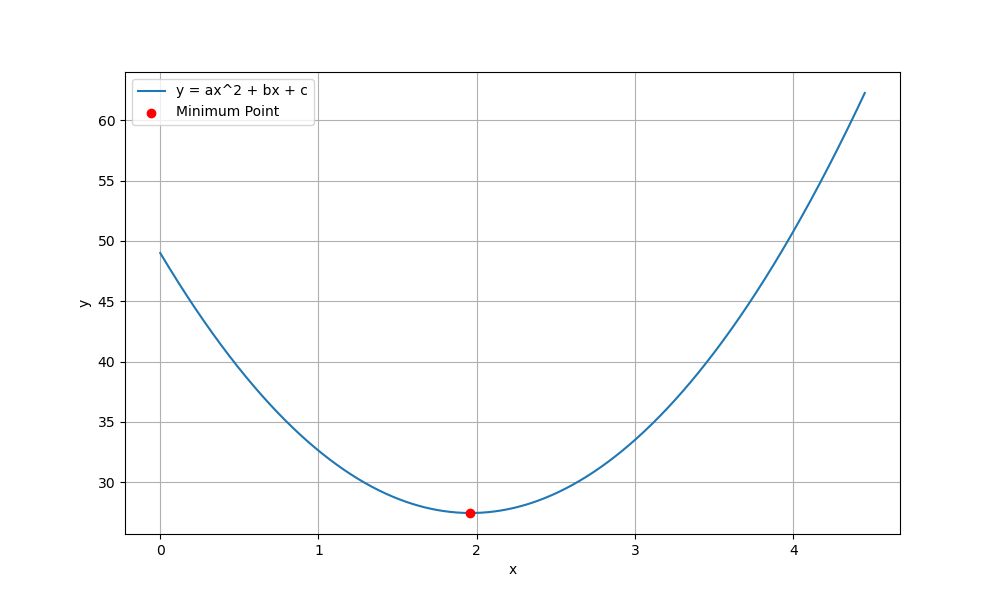
\includegraphics[width=1\columnwidth]{figs/fig.png}
   \caption{Minimum of the function}
\end{figure}
\end{frame}
\end{document}p
